\chapter{Step 02: Flip-Flops}
\label{ch:step02}

Step 01 had no memory: the LEDs showed a function of the buttons at that very
moment. Now we add state. The design of \cc{02_flip_flops} consists of two
flip-flops and the logic that computes their next values, a very small
\term{state machine}. The new piece of SystemVerilog is \cc{always_ff}.

\section{The Circuit}

Two D flip-flops store the bits $Q_1$ and $Q_2$. At every rising edge of the
clock they take over the values
\[
  Q_1' = \neg Q_1 \vee Q_2, \qquad Q_2' = \neg(Q_1 \wedge Q_2),
\]
which a combinational circuit computes from the current values. The outputs of
the flip-flops are fed back into this circuit (Figure~\ref{fig:step02-netlist}).

\begin{figure}[ht]
\centering
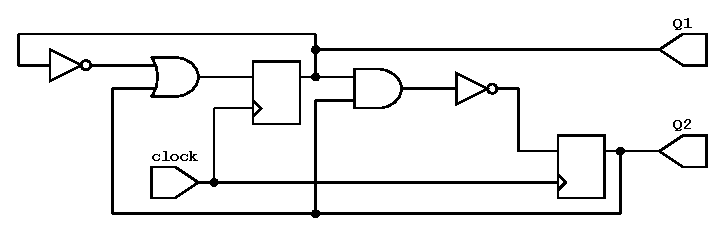
\includegraphics[width=0.85\linewidth]{figures/02_netlist.pdf}
\caption{The circuit of step 02, drawn by \cc{make svg}: two flip-flops (the
boxes with the small triangle at the clock input) and the logic between their
outputs and inputs.}
\label{fig:step02-netlist}
\end{figure}

Mathematically, the circuit is a map $\{0,1\}^2 \to \{0,1\}^2$, $(Q_1, Q_2)
\mapsto (Q_1', Q_2')$, which is applied once per clock cycle. Starting from
$(0,0)$ we get
\[
  (0,0) \mapsto (1,1) \mapsto (1,0) \mapsto (0,1) \mapsto (1,1) \mapsto (1,0)
  \mapsto \cdots
\]
After the first step, the state runs through a cycle of length three.

\section{The Description in SystemVerilog}

\svfile{02_flip_flops/test.sv}

\textbf{The combinational part} is an \cc{always_comb} block as in step 01. It
computes the two signals \cc{nextQ1} and \cc{nextQ2}, the inputs of the
flip-flops.

\textbf{\cc{always_ff} describes flip-flops.} The block
\begin{lstlisting}
always_ff @ (posedge clock) begin
    Q1 <= nextQ1;
    Q2 <= nextQ2;
end
\end{lstlisting}
says: at every rising edge (\cc{posedge}, positive edge) of \cc{clock}, \cc{Q1}
takes over the value of \cc{nextQ1}, and \cc{Q2} that of \cc{nextQ2}. Between
two rising edges they keep their values. That is the definition of a D
flip-flop with data input \cc{nextQ1}, output \cc{Q1}, and clock \cc{clock}.
So these three lines describe the two flip-flops of
Figure~\ref{fig:step02-netlist}.

\textbf{\cc{<=} is the non-blocking assignment.} In \cc{always_ff} we write
\cc{<=} instead of \cc{=}. Read \cc{Q1 <= nextQ1} as ``at the clock edge,
\cc{Q1} becomes what \cc{nextQ1} is just before the edge.'' All right-hand
sides in the block are taken from before the edge, and only then are all
flip-flops updated, at the same time. This is how real flip-flops behave: all
of them sample their inputs at the same edge.

The rule for the two kinds of blocks is simple, and we follow it in all
designs:
\begin{center}
\begin{tabular}{lll}
\toprule
block & describes & assignment \\
\midrule
\cc{always_comb} & combinational logic & \cc{=} \\
\cc{always_ff @ (posedge clock)} & flip-flops, updated at the rising edge & \cc{<=} \\
\bottomrule
\end{tabular}
\end{center}

\textbf{\cc{initial} sets the values at power-up.} The \cc{initial} block
states that \cc{Q1} and \cc{Q2} start as 0. On the FPGA this is the value the
flip-flops have right after the configuration is loaded. Our flip-flops start
with 0 anyway, so here it changes nothing on the chip, but it documents the
start state, and the simulation needs it (otherwise it would not know where to
start).

\textbf{The same type, two kinds of hardware.} \cc{nextQ1} and \cc{Q1} are
both declared as \cc{logic}. That \cc{nextQ1} becomes a wire and \cc{Q1} the
output of a flip-flop follows only from the block that assigns it. In
SystemVerilog, the hardware is determined by how a signal is used, not by its
declaration.

\begin{pitfall}
Assign every signal in \emph{one} block only. A signal that is assigned in an
\cc{always_comb} and also in an \cc{always_ff} would be the output of a gate
and of a flip-flop at the same time, two drivers on one wire. (The
\cc{initial} block is the one exception we allow ourselves: on the FPGA it sets
the power-up value of the flip-flop and drives nothing afterwards. Verilator's
linter does not know that and warns about it, see
Section~\ref{sec:step02-sim}.)
\end{pitfall}

\begin{exercise}
\label{ex:step02-blocking}
Swap the two lines in the \cc{always_ff} block. Does the circuit change? What
if the block were
\begin{lstlisting}
always_ff @ (posedge clock) begin
    Q1 <= ~Q1 | Q2;
    Q2 <= ~(Q1 & Q2);
end
\end{lstlisting}
without the \cc{always_comb} block?
\end{exercise}

\section{What yosys Makes of It}

The statistics in \cc{test.log} now list two kinds of building blocks:

\outputfile{step02_yosys_stat.txt}

An \cc{SB_DFF} is a D flip-flop, the one in a logic cell. Here is the netlist
in short, one building block per line with the signals at its connections
(\cc{C} clock, \cc{D} data input, \cc{Q} output; \cc{I0} to \cc{I3} and \cc{O}
for the LUTs):

\outputfile{step02_cells.txt}

Each next-state function became one LUT, whose output goes to the data input
of a flip-flop. Since a logic cell contains a LUT \emph{and} a flip-flop, nextpnr
puts each pair into one logic cell, and the whole design needs two of them (plus
two for the constants, as in step 01). You can check the LUTs as in
Section~\ref{sec:step01-yosys}: with \cc{Q2} on $x_3$ and \cc{Q1} on $x_2$, the
LUT of \cc{Q1} selects $t_{8Q_2 + 4Q_1}$, and its \cc{LUT_INIT} gives $t_0 = 1$,
$t_4 = 0$, $t_8 = t_{12} = 1$: that is $\neg Q_1 \vee Q_2$.

\section{How Fast May the Clock Be?}

Now there are paths from flip-flops through logic to flip-flops, and nextpnr can
say how long the slowest one takes. Its answer:

\outputfile{step02_pnr_fmax.txt}

With a clock of 232\,MHz there would still be enough time for the signal from
the output of a flip-flop through a LUT to the input of the next flip-flop. Our
board's clock has 12\,MHz, so there is plenty of room. That will change: the
ULM in Chapter~\ref{ch:step09} reaches only about 15\,MHz.

\section{Where Are the Pins?}
\label{sec:step02-pins}

nextpnr also prints warnings this time:

\outputfile{step02_pnr_warnings.txt}

The ports of this design are called \cc{clock}, \cc{Q1} and \cc{Q2}, and none
of these names is in \cc{icebreaker.pcf}. The Makefile calls nextpnr with
\cc{--pcf-allow-unconstrained}, so instead of an error we get these warnings,
and nextpnr connects the ports to \emph{some} pins. Moreover, the line
\cc{set_frequency CLK 12} in the pin file refers to \cc{CLK}, which does not
exist here, so nextpnr does not know which clock to check against. (It still
checks against 12\,MHz, its default.)

\begin{pitfall}
Port names of the top module must be names from \cc{icebreaker.pcf},
otherwise the port ends up on an arbitrary pin, and the design does nothing
visible on the board. Read the warnings of nextpnr: ``unconstrained in PCF''
always means a typo or a forgotten pin.
\end{pitfall}

To see something on the board, the ports need pin names. For the clock, the
12\,MHz oscillator \cc{CLK} is the obvious choice, but then the LEDs change
twelve million times per second, and you see them all glowing at the same time.
We need a slower clock, or a way to make something happen only once in a while.
This is what the next step is about.

\begin{exercise}
\label{ex:step02-button}
Rename the ports so that the first button is the clock and the LEDs show the
state: \cc{clock} becomes \cc{BTN1}, \cc{Q1} becomes \cc{LED1}, \cc{Q2} becomes
\cc{LED2} (also in the testbench). Program the board and press the button a few
times. Does the state always advance by one step per press?
\end{exercise}

\section{Simulation}
\label{sec:step02-sim}

The testbench now has only one input to set, the clock. Its loop inverts it in
every step:

\cpppart{firstline=21,lastline=30}{02_flip_flops/tb_test.cpp}

So the clock has a rising edge at every second step. Figure~\ref{fig:step02-waves}
shows the result of \cc{make sim} in the waveform viewer.

\begin{figure}[ht]
\centering
\begin{tikzpicture}[x=6.5mm,y=7mm]
  \foreach \name/\y in {clock/6, nextQ1/4.5, nextQ2/3, Q1/1.5, Q2/0} {
    \node[anchor=east,font=\small\ttfamily] at (-0.3,\y+0.3) {\name};
    \draw[black!8,line width=3mm] (0,\y+0.3) -- (15,\y+0.3);
  }
  % clock: 1 at t=0, toggles every step
  \draw[clocksig] (0,6.6) \foreach \t in {1,3,...,13} { -- (\t,6.6) -- (\t,6) -- (\t+1,6) -- (\t+1,6.6) } -- (15,6.6);
  % Q1: 0 until 2, 1 on [2,6), 0 on [6,8), 1 on [8,12), 0 on [12,14), 1 from 14
  \draw[signal] (0,1.5) -- (2,1.5) -- (2,2.1) -- (6,2.1) -- (6,1.5) -- (8,1.5) -- (8,2.1) -- (12,2.1) -- (12,1.5) -- (14,1.5) -- (14,2.1) -- (15,2.1);
  % Q2: 0 until 2, 1 on [2,4), 0 on [4,6), 1 on [6,10), 0 on [10,12), 1 on [12,16)
  \draw[signal] (0,0) -- (2,0) -- (2,0.6) -- (4,0.6) -- (4,0) -- (6,0) -- (6,0.6) -- (10,0.6) -- (10,0) -- (12,0) -- (12,0.6) -- (15,0.6);
  % nextQ1 = ~Q1 | Q2: 1 on [0,4), 0 on [4,6), 1 on [6,10), 0 on [10,12), 1 on [12,...)
  \draw[signal,draw=green!45!black] (0,5.1) -- (4,5.1) -- (4,4.5) -- (6,4.5) -- (6,5.1) -- (10,5.1) -- (10,4.5) -- (12,4.5) -- (12,5.1) -- (15,5.1);
  % nextQ2 = ~(Q1 & Q2): 1, 0 on [2,4), 1 on [4,8), 0 on [8,10), 1 on [10,14), 0 on [14,...)
  \draw[signal,draw=green!45!black] (0,3.6) -- (2,3.6) -- (2,3) -- (4,3) -- (4,3.6) -- (8,3.6) -- (8,3) -- (10,3) -- (10,3.6) -- (14,3.6) -- (14,3) -- (15,3);
  \foreach \t in {0,2,...,14} {
    \draw[black!12] (\t,-0.4) -- (\t,6.9);
    \node[below,font=\scriptsize] at (\t,-0.4) {\t};
  }
  \node[note,anchor=west] at (15.3,-0.7) {\cc{sim_time}};
\end{tikzpicture}
\caption{The waveforms of step 02. At every rising edge of \cc{clock} (the
gray lines), \cc{Q1} and \cc{Q2} take over the values that \cc{nextQ1} and
\cc{nextQ2} had just before.}
\label{fig:step02-waves}
\end{figure}

The simulation starts at time 0 with \cc{clock} already 1. This is not a rising
edge, since there is no earlier value, so the state stays $(0,0)$. The first
rising edge is at time 2, and from there on the state runs through $(1,1)$,
$(1,0)$, $(0,1)$, $(1,1)$, \dots, as computed above. Note how \cc{nextQ1} and
\cc{nextQ2} change right after an edge, as soon as the state has changed: they
are combinational, and they always show what the state will be after the next
edge.

Verilator prints some warnings during \cc{make sim}:
\begin{terminal}
%Warning-MULTIDRIVEN: test.sv:20:9: Variable written to in always_ff also
written by other process (IEEE 1800-2023 9.2.2.4): 'Q1'
\end{terminal}
This is the \cc{initial} block of the pitfall above. For a simulator, it is a
second process writing \cc{Q1}. For us, it is the power-up value of the
flip-flop, and we can ignore the warning.

\solutions

\solution
Swapping the lines changes nothing: both right-hand sides are taken from before
the edge, and both flip-flops are updated together. The order of the lines in
an \cc{always_ff} block with \cc{<=} does not matter.

The block without \cc{always_comb} describes the same circuit as well. The
expressions on the right are computed by combinational logic in any case; we
only no longer give its outputs names. Here, \cc{Q1} on the right of the second
line is still the old value, since \cc{<=} takes all right-hand sides from
before the edge. (With \cc{=} instead of \cc{<=}, the second line would see the
new value of \cc{Q1}, and the block would describe a different circuit. This
is why we never use \cc{=} in \cc{always_ff}.)

\solution
After renaming, nextpnr finds all ports in the pin file, and the warnings are
gone. On the board you will see the state advance, but now and then by two or
more steps per press. A mechanical button does not close cleanly: its
contacts bounce for a few milliseconds and produce several edges. For a clock,
which must be clean, a button is a bad choice. We will instead sample buttons
with the 12\,MHz clock, starting in Chapter~\ref{ch:step04}, and react to a
press only once the contacts have settled, starting in
Chapter~\ref{ch:step05}.
